
\section{MIC implementation}
One of the most important factors to take into consideration when implementing PV modules is to constantly obtain the maximum energy possible out of these PV panels. If this is not done, the amount of energy that should have been obtained will instead be lost. Since energy is equal to power over time, power must be maximized when the energy is being extracted. To achieve such goal a MPPT needs to be implemented. This is an electrical system that is always on the search of the location of the MPP where the power generated by the PV module is maximum. MPPTs mostly consist of a power circuit that regulates either voltage drop or current flow across the PV terminals. There are different kinds of circuits that can be used to follow the MPP of the PV, this topic will be further introduced in chapter \ref{background}.

Solar plants and domestic installations are composed of several modules connected to each other in series or parallel configurations. To simplify the PV system's structure, one MPPT is commonly used for many modules as shown in figure \ref{fig:PVsystemblocks}. This approach may lead to unoptimal efficiency of the system since the uneven power generated by the PV modules might lead to have a system with a local MPP in addition to a global MPP \cite{AN1521_MC}. In figure \ref{multiple_local_MPP} a system exhibiting two MPP, due to partial shading, is shown. In order to ensure that the system is working in the global MPP and not in the local MPP, the controller will have to perform a voltage sweep in order to find the global MPP. This voltage sweep is a higher level of complexity in the MPPT control system \cite{AN1521_MC}. In any case, the system will not be able to get the maximum power generation, as one panel is bypassed by a diode.

\begin{figure}[htbp]
	\begin{center}
		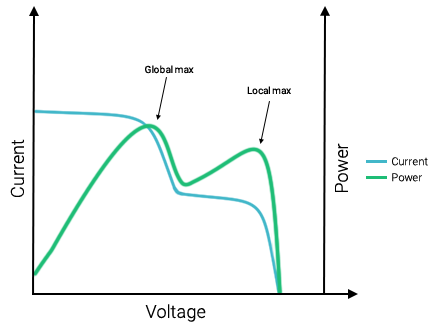
\includegraphics[width=0.6\textwidth]{../Pictures/local_MPP}
		\caption{I-V curve of a system with more than one MPP \cite{local_mpp}.}
		\label{multiple_local_MPP}
	\end{center}	
\end{figure}

Another possible configuration is using MICs for each PV module which will result in higher overall efficiencies \cite{ArchitectureMIC}. With this configuration, events like partial shading, uneven dirt, wear distribution or imperfections produced during the assembly line are reduced and do not affect the rest of the PV modules in the array. Also, a more detailed control of the plant is achieved since separate data from each individual panel is obtained \cite{ArchitectureMIC}.
As seen so far, different implementation options for MIC devices are possible but the most important objective of these devices is to individually control each PV module, resulting in an overall improved efficiency as well as a more robust system against any kind of disturbance \cite{ArchitectureMIC}. Each PV module will then be connected directly to a MIC allowing the output voltage and current to be defined by the load, either an inverter or a battery.  This way the system is able to operate at different voltage and current levels whilst maintaining the MPP at all time \cite{ArchitectureMIC}. 

MICs can be either microinverters or DC-DC converters. In figure \ref{MIC_dcdc} a PV system using MICs to perform the voltage reduction or increase is used. Notice that $N$ panels might be used. Series or parallel connections can be used to link MICs' outputs and then connect this output to the inverter input through a DC link.  The power rating of this inverter will have to be higher than the maximum power that can be delivered by MICs. Then the size of the inverter must consider the amount of PV panels installed.

\begin{figure}[H]
	\begin{center}
		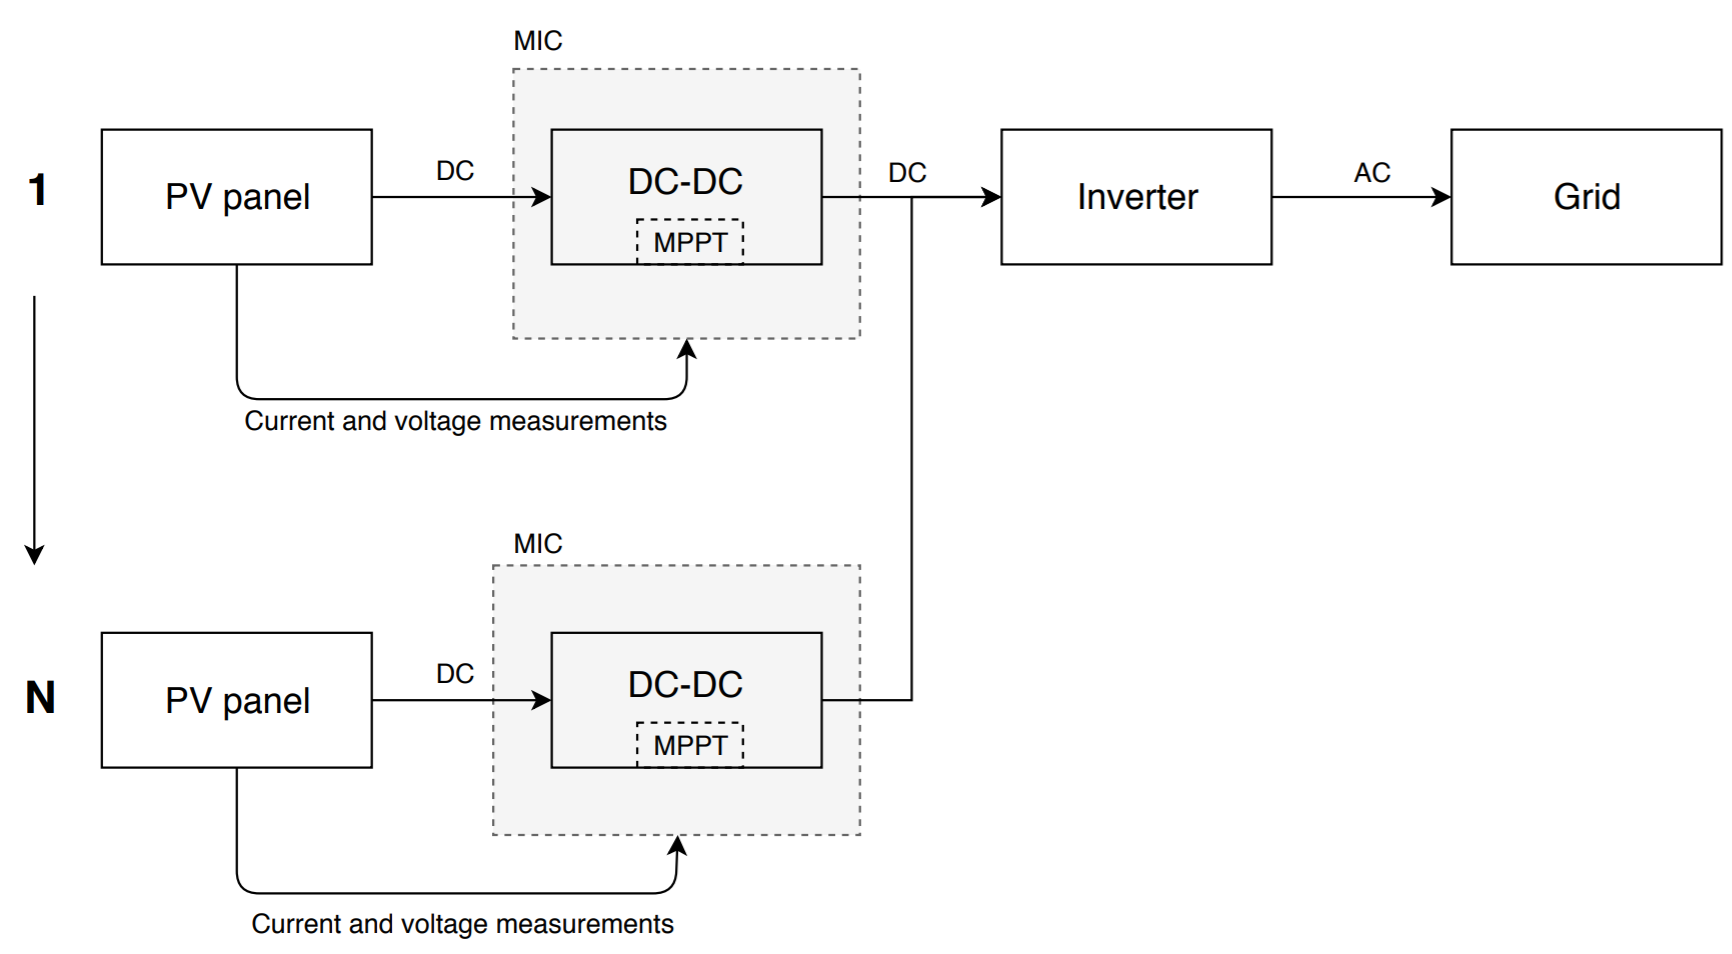
\includegraphics[width=0.7\textwidth]{../Pictures/MIC_dcdc}
		\caption{PV generation with DC-DC MIC system structure.}
		\label{MIC_dcdc}
	\end{center}	
\end{figure}

The panels with a MIC consisting on a microinverter, include a DC-DC converter with MPPT together with an inverter and are directly tied to grid. In figure \ref{microinverter_system} a microinverter system structure can be seen. For the user, this system is simpler, as only the PV must be purchased. The user doesn't have to worry about selecting and installing an inverter. 

\begin{figure}[H]
	\begin{center}
		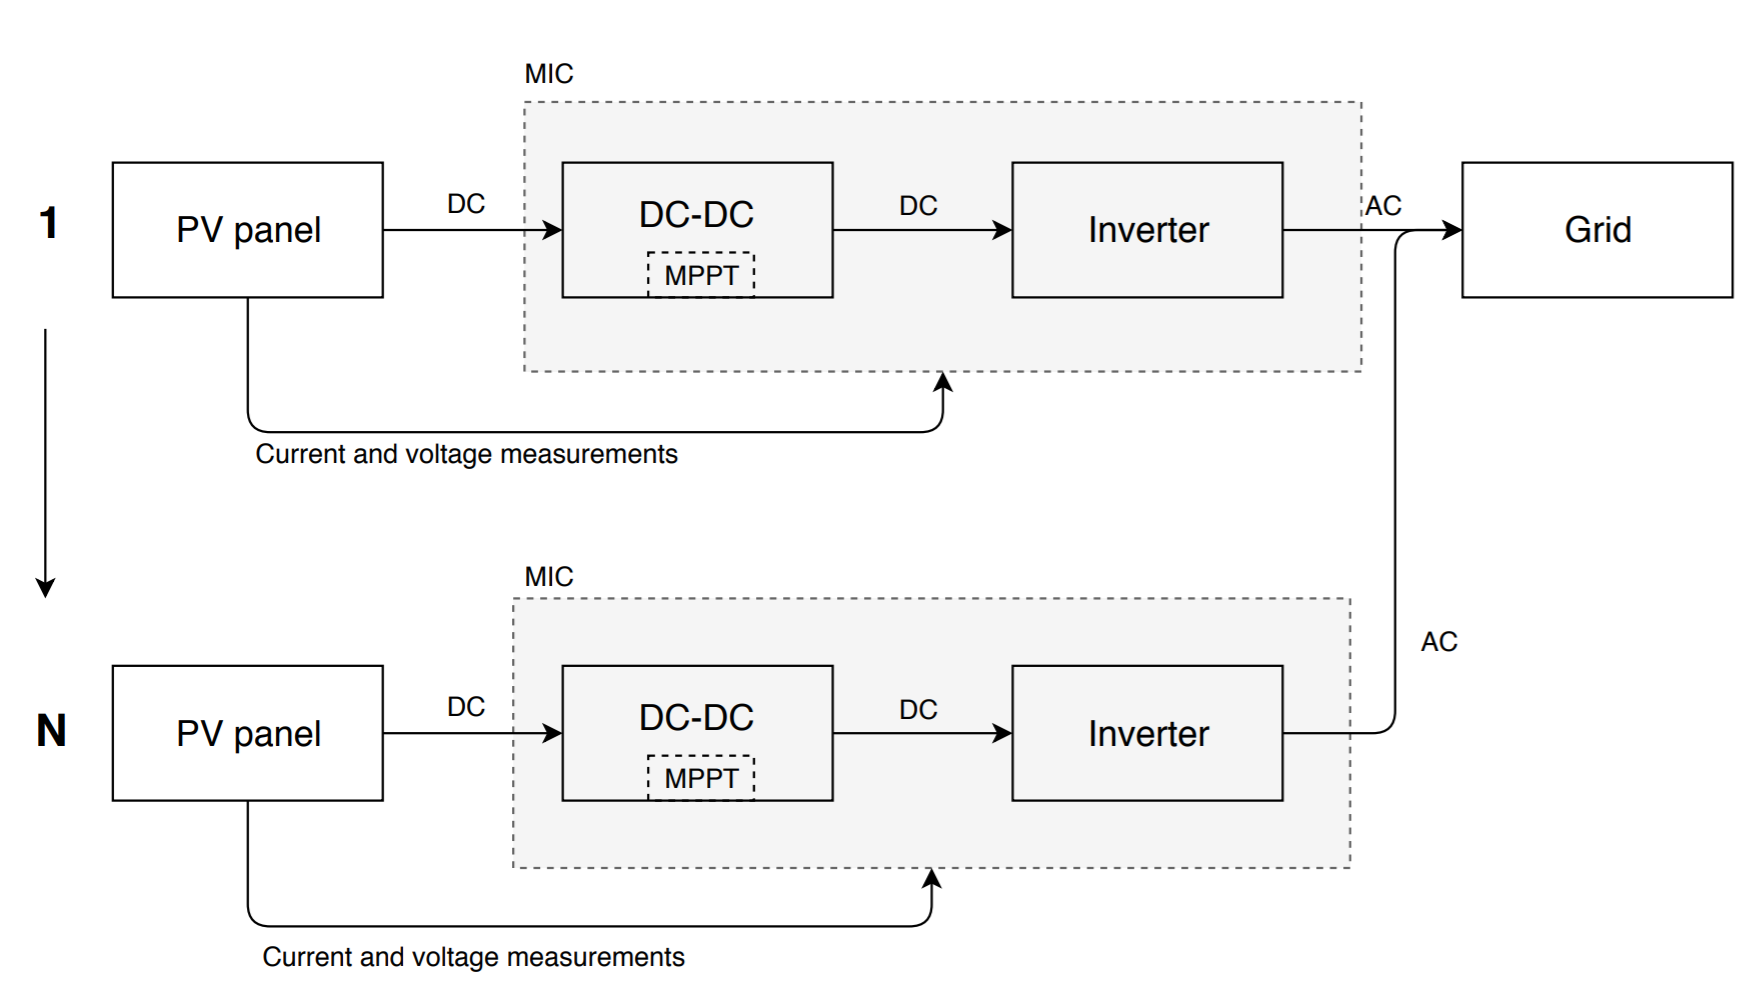
\includegraphics[width=0.7\textwidth]{../Pictures/MIC_microinverter}
		\caption{PV generation with microinverter MIC system structure.}
		\label{microinverter_system}
	\end{center}	
\end{figure}

The main advantage of the microinverter system is that it is simpler for the user, however, it implies an increase in costs and are usually less efficient than a DC-DC system with a higher power general inverter \cite{ArchitectureMIC}. Therefore, for the development of this project a DC-DC MIC will be employed. 


